% docs/extended_abstract/extended_abstract.tex
%
% Extended abstract assembled VERBATIM from the project's public data page
% (www/data.html). No text below was authored for this document; typos and
% phrasing are reproduced as they appear on the site. Maps rendered by
% make_maps.R from the tract-level estimates. The abstract (abstract.tex) and
% any citations are the author's own; build with build.sh.

\documentclass[11pt]{article}
\usepackage[margin=0.9in]{geometry}
\usepackage{amsmath, amssymb}
\usepackage{setspace}
\usepackage{graphicx}
\usepackage{pdflscape}
\usepackage{enumitem}
\usepackage[authoryear,round]{natbib}   % \citet{key} / \citep{key}; keys in references.bib
\usepackage[hidelinks]{hyperref}
\usepackage{textcomp}
\setstretch{1.12}
\setlist[itemize]{leftmargin=1.4em, itemsep=0.35em}

\title{Gaydar: Estimating Local LGBTQ Populations}
\author{Nicholas Martens}
\date{}

\begin{document}
\maketitle

\begin{abstract}
How many LGBTQ people live in your neighborhood? Measurement of the LGBTQ community is notoriously challenging, particularly with any degree of geographic granularity. I produce tract-level estimates of non-binary (NB) and lesbian and gay, bisexual, transgender, and queer (LGBTQ) populations from publicly available US Census Bureau data. Foremost, I capture the spatial variation in the levels and concentration of NB and LGBTQ people, with separate estimates by gender identity for lesbians and gay, bisexual, and queer people. Hence, the estimates incorporate within-cohort variation in sexual orientation across different gender identities. I also capture local variation in the cross-sectional composition of the LGBTQ community (for example, bisexuals and queers comprise more of the community in college-student heavy tracts). Finally, I incorporate measures of uncertainty into the estimates, reflecting sampling variation across multiple Census data products. The estimates offer insights for scholars of LGBTQ demographics, public health practitioners, and myriad others.    % edit abstract.tex, not this block
\end{abstract}

Gaydar explores the spatial distribution of non-binary (NB) and/or gay and lesbian, bisexual, transgender, and queer (LGBTQ) people. I focus on adult (18+) NB and LGBTQ (sorry asexuals), split into three mutually exclusive and collectively exhaustive gender identities: men, women, and non-binary people.

To view the results of the estimation methodology described below, use 
\href{https://martensn.shinyapps.io/gaydar/}{this interactive map}.

Note transgender people might also identify as gay, lesbian, bisexual, or
queer, meaning the sub-population shares will not sum to the total because I
don't double count LGBQ transgender people. Additionally, limitations within
Household Pulse Survey microdata mean that I cannot measure non-binary
transgender individuals.

\section*{Summary}

\begin{itemize}
\item Estimate LGBTQ identification rates by state $\times$ sex assigned at
  birth $\times$ age bin using pooled Household Pulse Survey (HPS) microdata,
  with survey-weighted estimation and soft calibration to recent Gallup
  national benchmarks.

\item Estimate gender identity composition conditional on sexual orientation,
  sex assigned at birth, and age, using HPS microdata to recover age-specific
  distributions of different gender identities. I assume cisgender,
  non-binary, and transgender are mutually exclusive and collectively
  exhaustive. Step 2 constructs a crosswalk from ACS age-sex counts to
  age-gender identity-sexuality estimates. These composition estimates are
  stabilized using age-local Dirichlet smoothing, allowing gender identity
  shares to vary smoothly across cohorts while remaining responsive to
  well-identified age groups (For example, younger AFAB lesbians roughly 15
  percentage points more likely to identify as non-binary than AMAB gays in
  the same age cohort. Age-local Dirichlet smoothing preserves the pattern,
  just smoothing out some of the noise).

\item Estimate LGBTQ sub-population shares (i.e. lesbians and gays, bisexuals,
  queers, transgender people) by pooling nationally rather than by state.
  State-level cells (think transgender people in any state or bisexuals in
  Wyoming) were too sparse to trust even with empirical Bayes shrinkage
  across states, so every state now applies the same national
  LG/bisexual/queer mix to its own state-level identification rate from
  step 1.

\item Project expected LGBTQ population counts to Census tracts by combining
  estimated identification rates with ACS 5-year age--sex population counts
  (table B01001). Since age and sex vary locally, sexuality and gender
  identity will too.

\item Reweight projected LGBTQ populations within states by blending two
  PUMA-level spatial proxies: the observed concentration of same-sex couples,
  and the observed concentration of singles within the same birth sex and
  age cell. Note that same-sex couples tend to be older, wealthier, better
  educated, and more likely to identify as gay or lesbian than the broader
  LGBTQ population \citep{julian2024a}, which suggests their spatial concentration patterns might
  systematically differ --- especially for young, non-binary, and transgender
  people, who are least likely to show up as a Census-visible couple at all \citep{gates2013}.
  I address this by blending in the concentration of singles of the same sex
  and age, weighted by that cell's HPS-estimated marriage rate: cells that
  are more often married lean on the couples signal, cells rarely married
  lean on the singles signal instead. Nonetheless, the reweighting ensures
  the estimates reflect more than the age and sex composition of a Census
  tract.

  The reweighting produces a calibration factor for each PUMA, but applying
  that factor as a hard step function at PUMA boundaries introduces visual
  discontinuities in the map that are artifacts of the PUMA delineation
  rather than real demographic transitions. To address this, I smooth the
  calibration factors to the tract level using inverse-distance weighting
  (IDW): each tract receives a distance-weighted blend of all PUMA factors
  rather than the factor of whichever PUMA it happens to fall in. This
  preserves the geographic heterogeneity the calibration is meant to capture
  while producing a spatially continuous surface.

\item Enforce a capacity constraint so that no tract's LGBTQ estimate exceeds
  its gender-group population. In high-concentration areas, the reweighting
  and rescaling can push estimates above 100 percent of the relevant
  gender-group total. I cap each gender group's estimates at its population
  and scale sub-populations (lesbian/gay, bisexual, queer, transgender) down
  proportionally, preserving within-group composition.
\end{itemize}

\section*{Data Sources}

\subsection*{Household Pulse Survey (HPS)}

HPS was the first the Census data product to ask respondents about sexual
orientation and gender identity, basing the design of questions on the
results of a 2022 NASEM report \citep{nasem2022}. Designed to elicit responses to rapidly
changing situations (i.e. food security early in the coronavirus pandemic),
the HPS surveyed different households each week. While topics varied between
weeks, HPS consistently collected the following demograhic data:

\begin{itemize}[itemsep=0.1em]
\item Sexual orientation
\item Gender identity
\item Sex assigned at birth
\item Year of birth
\item Marital status
\item State of residence
\item Survey weights
\end{itemize}

The microdata allow the relationship between sexual orientation and gender
identity to vary flexibly by age and geography. For example, younger gay and
lesbian individuals are more likely to identify as non-binary than older
cohorts.

\subsection*{Gallup Polling}

The February 2026 Gallup report provides the most recent nationally
representative estimate of LGBTQ identification in the United States.

The report includes:

\begin{itemize}[itemsep=0.1em]
\item Overall national LGBTQ identification
\item LGBTQ identification by generation
\item LGBTQ identification by generation $\times$ sex (for select cohorts)
\end{itemize}

Given uncertainty in survey measurement, these estimates are used as soft
calibration targets, not hard constraints. In practice, most state-level
estimates fall within one to two percentage points of Gallup's top-line
estimate of 9 percent.

\subsection*{American Community Survey (ACS)}

Population projections are anchored to ACS 5-year estimates, which provide
stable small-area population counts at fine geographic resolution.

Specifically, the pipeline uses:

\begin{itemize}[itemsep=0.1em]
\item Table B01001 (Sex by Age) to obtain population counts by sex assigned at
  birth and granular age bins, measured at the tract level.
\item Table B09019 (Household Type by Relationship) informs the
  same-sex-couples half of the spatial reweighting above, measured at the
  PUMA level.
\item Table B12002 (Sex by Marital Status by Age) provides the
  singles-concentration signal blended into the same reweighting, also
  measured at the PUMA level.
\end{itemize}

Because the Household Pulse Survey (HPS) and ACS use different age groupings,
HPS respondents are mapped into ACS-compatible age bins prior to estimation.
This ensures that estimated LGBTQ identification rates and gender-composition
shares can be directly applied to ACS population counts without interpolation
or extrapolation.

\newgeometry{margin=0.4in}
\begin{landscape}
\thispagestyle{empty}
\null\vfill
\begin{center}
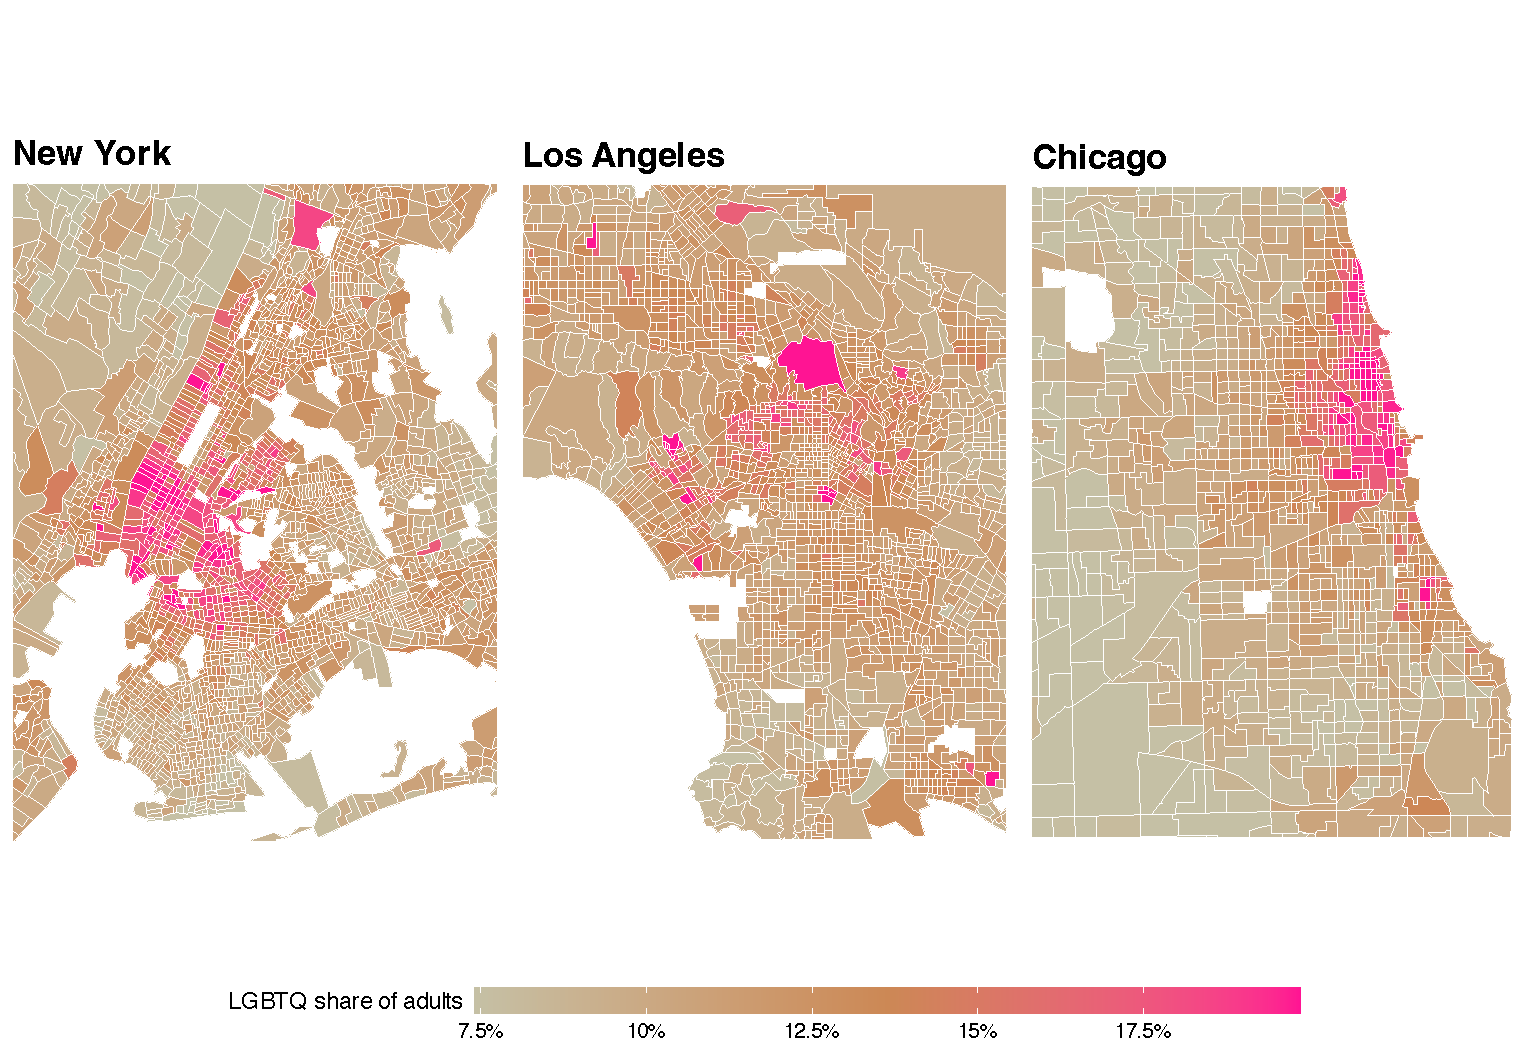
\includegraphics[width=\linewidth,height=0.96\textheight,keepaspectratio]{figs/maps_three_cities.pdf}
\end{center}
\vfill
\end{landscape}
\restoregeometry

% References. The heading only appears once something is cited (bibtex emits
% an empty list otherwise). AER style: author-year in text, alphabetical list.
\bibliographystyle{aer}
\bibliography{references}

\end{document}
